\documentclass[10pt]{article}
\usepackage[utf8]{inputenc}
\usepackage[doublespacing]{setspace}
\usepackage{textcomp}
\usepackage{amsmath,amssymb,amsthm}
\usepackage{fancyhdr}
\usepackage{lastpage}
\usepackage[]{hyperref}
\usepackage[pdftex]{graphicx}
\usepackage{ctex}
\usepackage{booktabs}
\usepackage{subfigure}
\usepackage{titlesec}
\usepackage{listings}
\usepackage{enumerate}
\usepackage{bm}
\usepackage{float}
\usepackage{url}
%\allowdisplaybreaks
\renewcommand{\contentsname}{\centerline{Contents}}
\pagestyle{fancy}
\author{D}
\def\name{D}
\lhead{Time Series Methods}
\chead{}
\rhead{\name}
\cfoot{-\space\thepage\space-}
\newtheorem{exer}{\bm{$Exercise$}}
\newtheorem{prob}{\bm{$Problem$}}
\newtheorem{bonus}{\bm{$Bonus\;Problem$}}
\newcommand{\tabincell}[2]{\begin{tabular}{@{}#1@{}}#2\end{tabular}}
\CTEXoptions[today=old]

\begin{document}

\title{Assignment Four}
\date{\today}
\maketitle
\thispagestyle{fancy}
\thispagestyle{fancy}

\begin{prob}
\end{prob}
\begin{enumerate}[1)]
\vspace{3mm}

\item
AR(1): $X_t=0.7X_{t-1}+W_t$\\
Using the backshift operator, we have the expression,
\begin{align*}
X_t-0.7X_{t-1}&=W_t\\
X_t-0.7BX_t&=W_t\\
(1-0.7B)X_t&=W_t.
\end{align*}
The characteristic polynomial is
\begin{align*}
\phi(B)&=1-0.7B\\
\phi(z)&=1-0.7z.
\end{align*}
When $\phi(z)=0$,
\begin{align*}
1-0.7z&=0\\
z&=\frac{10}{7}.
\end{align*}
So we have
\begin{align*}
\phi_1&=0.7,\\
|z|=\frac{10}{7}&>1.
\end{align*}
To meet the stationarity, $|z|\neq1$; to meet the causality, $|\phi_1|<1$ or $|z|>1$.\\
Hence, the process satisfies both conditions, and is causal stationary.

\item
MA(2): $X_t=W_t-1.2W_{t-1}+0.35W_{t-2}$\\
Using the backshift operator, we have the expression,
\begin{align*}
X_t&=W_t-1.2BW_t+0.35B^2W_t\\
X_t&=(1-1.2B+0.35B^2)W_t.
\end{align*}
The characteristic polynomial is
\begin{align*}
\theta(B)&=1-1.2B+0.35B^2\\
\theta(z)&=1-1.2z+0.35z^2.
\end{align*}
When $\theta(z)=0$,
\begin{align*}
1-1.2z+0.35z^2&=0\\
z&=\frac{-(-1.2)\pm\sqrt{(-1.2)^2-4*1*0.35}}{2*0.35}\\
z&=\frac{1.2+\sqrt{\frac{36}{25}-\frac{7}{5}}}{\frac{7}{10}}\;\textrm{or}\;\frac{1.2-\sqrt{\frac{36}{25}-\frac{7}{5}}}{\frac{7}{10}}\\
z&=2\;\textrm{or}\;\frac{10}{7}.
\end{align*}
So we have
\begin{align*}
|z|=2\;\textrm{or}\;\frac{10}{7}&>1.
\end{align*}
To meet the invertibility, $|z|>1$.\\
Hence, both the absolute values of the two roots of z are greater than 1, the process satisfies the condition and is invertible.

\item
AR(2): $X_t=1.8X_{t-1}-0.81X_{t-2}+W_t$\\
Use the backshift operator, we have the expression,
\begin{align*}
X_t-1.8X_{t-1}+0.81X_{t-2}&=W_t\\
X_t-1.8BX_t+0.81B^2X_t&=W_t\\
(1-1.8B+0.81B^2)X_t&=W_t.
\end{align*}
The characteristic polynomial is
\begin{align*}
\phi(B)&=1-1.8B+0.81B^2\\
\phi(z)&=1-1.8z+0.81z^2.
\end{align*}
When $\phi(z)=0$,
\begin{align*}
1-1.8z+0.81z^2&=0\\
z&=\frac{-(-1.8)\pm\sqrt{(-1.8)^2-4*1*0.81}}{2*0.81}\\
z&=\frac{1.8+\sqrt{\frac{81}{25}-\frac{81}{25}}}{\frac{81}{50}}\;\textrm{or}\;\frac{1.8-\sqrt{\frac{81}{25}-\frac{81}{25}}}{\frac{81}{50}}\\
z&=\frac{10}{9}.
\end{align*}
So we have
\begin{align*}
|z|=\frac{10}{9}&>1.
\end{align*}
To meet the stationarity, $|z|\neq1$; to meet the causality, $|z|>1$.\\
Hence, the process satisfies the two conditions and is causal stationary.

\end{enumerate}
\vspace{3mm}

\begin{prob}
\end{prob}
\vspace{3mm}
\begin{proof}
AR(3): $X_t=X_{t-1}+\phi{X_{t-2}}-\phi{X_{t-3}}+W_t$\\
Using the backshift operator, we have the expression,
\begin{align*}
X_t-X_{t-1}-\phi{X_{t-2}}+\phi{X_{t-3}}&=W_t\\
X_t-BX_t-\phi{B^2}X_t+\phi{B^3}X_t&=W_t\\
(1-B-\phi{B^2}+\phi{B^3})X_t&=W_t.
\end{align*}
The characteristic polynomial is
\begin{align*}
\phi'(B)&=1-B-\phi{B^2}+\phi{B^3}\\
\phi'(z)&=1-z-\phi{z^2}+\phi{z^3}.
\end{align*}
Let $z_1$, $z_2$ and $z_3$ be the roots of the characteristic polynomial.\\
Also, assume that the AR(3) process is causal stationary, so we have $|z_1|>1$, $|z_2|>1$ and $|z_3|>1$.\\
When $z=1$, $\phi'(z)=1-z-\phi{z^2}+\phi{z^3}=1-1-\phi+\phi=0$. Hence, $1$ is one of the roots of the polynomial, i.e. $|z_1|=1$, $|z_2|=1$ or $|z_3|=1$.\\
They contradict. The assumption does not hold.\\
Therefore, the AR(3) process $X_t=X_{t-1}+\phi{X_{t-2}}-\phi{X_{t-3}}+W_t$ is not causal stationary.
\end{proof}
\vspace{3mm}

\begin{prob}
\end{prob}
\begin{enumerate}[1)]
\vspace{3mm}

\item
AR(2):$X_t=\phi_1X_{t-1}+\phi_2X_{t-2}+W_t$\\
Use the backshift operator, we have the expression,
\begin{align*}
X_t-\phi_1X_{t-1}-\phi_2X_{t-2}&=W_t\\
X_t-\phi_1BX_t-\phi_2B^2X_t&=W_t\\
(1-\phi_1B-\phi_2B^2)X_t&=W_t.
\end{align*}
The characteristic polynomial is
\begin{align*}
\phi'(B)&=1-\phi_1B-\phi_2B^2\\
\phi'(z)&=1-\phi_1z-\phi_2z^2.
\end{align*}
When $\phi'(z)=0$,
\begin{align*}
1-\phi_1z-\phi_2z^2&=0\\
z&=\frac{-(-\phi_1)\pm\sqrt{(-\phi_1)^2-4*1*(-\phi_2)}}{2*(-\phi_2)}\\
z&=\frac{\phi_1\pm\sqrt{\phi_1^2+4\phi_2}}{-2\phi_2}
\end{align*}
Inspired by Part 3, Problem 1, where $\phi_1=1.8$ and $\phi_2=-0.81$, we can have $\phi_1=1.6$ and $\phi_2=-0.64$ in this case,
\begin{align*}
z&=\frac{1.6\pm\sqrt{1.6^2+4(-0.64)}}{2*0.64}\\
z&=\frac{1.6+\sqrt{1.6^2+4(-0.64)}}{2*0.64}\;\textrm{or}\;\frac{1.6-\sqrt{1.6^2+4(-0.64)}}{2*0.64}\\
z&=1.25
\end{align*}
So we have
\begin{align*}
|z|=1.25&>1.
\end{align*}
To meet the causal stationarity, $|z|>1$.\\
Hence, the AR(2) process $X_t=1.6X_{t-1}-0.64X_{t-2}+W_t$ is causal stationary.

\item
AR(2): $X_t=1.6X_{t-1}-0.64X_{t-2}+W_t$\\
R codes:
\lstinputlisting{p32a.R}
R outputs:
\lstinputlisting{p32a.txt}
\begin{figure}[H]
  \centering
  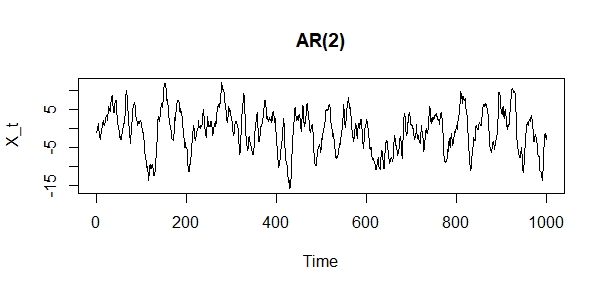
\includegraphics[width=10cm,height=5cm]{p32a.jpeg} % Comment: features of this plot?
  %\caption{}
\end{figure}
\begin{figure}[H]
  \centering
  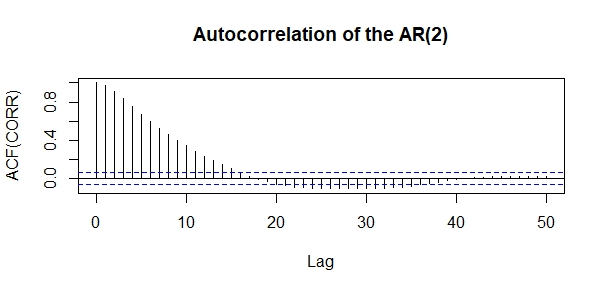
\includegraphics[width=10cm,height=5cm]{p32b.jpeg}
  %\caption{}
\end{figure}
Features:\\
The AR(2) process is stationary.\\
The theoretical mean is 0; the theoretical variance is $\frac{(1-(-0.64)*1)}{(1-0.64)[(1-(-0.64))-1.6^2]}=\frac{25625}{729}$.\\
The sample mean is -0.4977; the sample variance is 29.35015.\\
The theoretical autocovariance function is
\begin{align*}
\gamma(h)&=\left\{\begin{array}{ll}VAR[X_t]=\frac{25625}{729},\textrm{if}\;h=0,\\
\frac{1.6}{1-(-0.64)}\gamma(0)=\frac{25000}{729},\;\textrm{if}\;|h|=1,\\
1.6\gamma(h-1)-0.64\gamma(h-2),\;\textrm{if}\;|h|>1.\end{array}\right.
\end{align*}
The theoretical autocorrelation function is
\begin{align*}
\rho(h)&=\left\{\begin{array}{ll}1,\textrm{if}\;h=0,\\
\frac{25000}{25625}=\frac{40}{41},\;\textrm{if}\;|h|=1,\\
\frac{1.6\gamma(h-1)-0.64\gamma(h-2)}{\gamma(0)},\;\textrm{if}\;|h|>1.\end{array}\right.
\end{align*}
The theoretical autocorrelation decreases from 1 to 0, being always positive. Starting from 30 lags, it is almost zero.\\
The sample autocorrelation function, with its key values and plots, is shown in the outputs. The sample autocorrelation decreases from 1 lag to approximately 26 lags, being negative since approximately 18 lags, and then increases to 0 since 27 lags and stays around 0 since 40 lags.

\item
The theoretical partial autocorrelation function is
\begin{align*}
\phi'_{hh}&=\left\{\begin{array}{ll}\rho(1)=\frac{40}{41},\textrm{if}\;|h|=1,\\
\phi(2)=-0.64,\textrm{if}\;|h|=2,\\
0,\;\textrm{if}\;|h|>2.\end{array}\right.
\end{align*}
R codes:
\lstinputlisting{p33a.R} % Comment: Code from lab can do this in 1 line. You are allowed to use this.
R outputs:
\lstinputlisting{p33a.txt}
\begin{figure}[H]
  \centering
  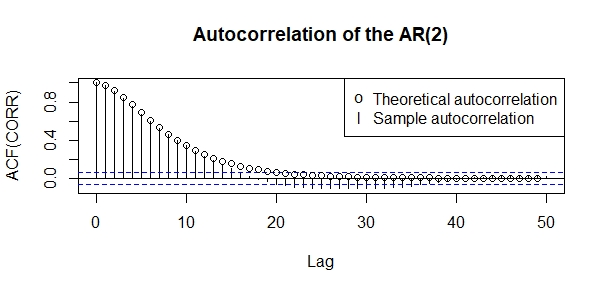
\includegraphics[width=10cm,height=5cm]{p33a.jpeg}
  %\caption{}
\end{figure}
\begin{figure}[H]
  \centering
  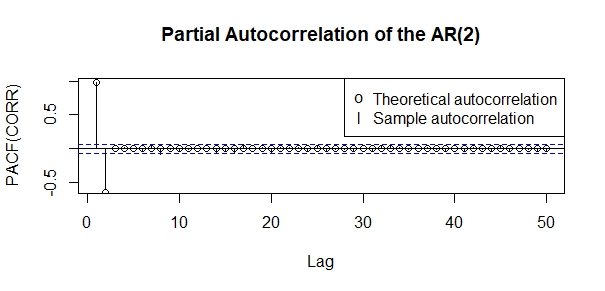
\includegraphics[width=10cm,height=5cm]{p33b.jpeg}
  %\caption{}
\end{figure}

\item
R codes:
\lstinputlisting{p34a.R}
The OLS method:\\
R outputs:
\lstinputlisting{p34a.txt}
The method of moments:\\
R codes:
\lstinputlisting{p34b.txt}
Comparison:\\
Using the OLS method, we get $\hat{\phi}_1=1.54807$ and $\hat{\phi}_2=-0.59309$.\\
Using the method of moments, we get $\hat{\phi}_1=1.5433089$ and $\hat{\phi}_2=-0.5889001$.\\
The real coefficients are $\phi_1=1.6$ and $\phi_2=-0.64$.

Why not the same?\\
Through the different theoretical and sample means and variances in Part 2, Problem 3, we know that the randomly generated AR(2) data is not strictly on the original AR(2) time series. So the estimation made through the data must be biased.\\
The OLS method has some defects, such as outliers, dependence among variables, wrong choices of error functions, heteroskedasticity and noise in the independent variables, which may cause the bias.\footnote{ ClockBackward. (2009). \textit{Ordinary least squares linear regression: flaws, problems and pitfalls}. Retrieved from \url{https://lcn.people.uic.edu/classes/che205s17/docs/che205s17_reading_06c.pdf}.}\\
The method of moments yields consistent estimators (under very weak assumptions) and these estimators are often biased. The method of moments does not rely on the infrequent with large samples but not so infrequent with small samples, so the estimates given by the method of moments can be outside of the parameter space.\footnote{ Wikipedia contributors. (2019). Method of moments (statistics). \textit{Wikipedia, the free encyclopedia}. Retrieved from \url{https://en.wikipedia.org/w/index.php?title=Method_of_moments_(statistics)&oldid=904795922}.}

\end{enumerate}
\vspace{3mm}

\begin{prob}
\end{prob}
\begin{enumerate}[1)]
\vspace{3mm}

\item
R codes:
\lstinputlisting{p41a.R}
R outputs:
\lstinputlisting{p41a.txt}
\begin{figure}[H]
  \centering
  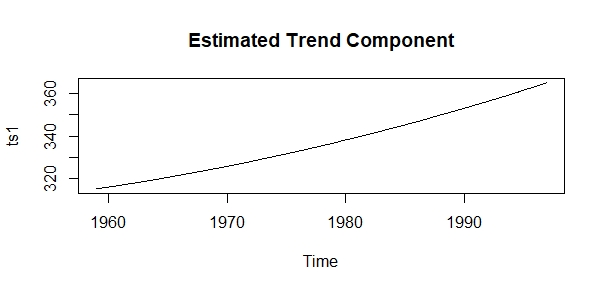
\includegraphics[width=10cm,height=5cm]{p41a.jpeg} % Comment: Only need one model with both trend and seasonality in.
  %\caption{}
\end{figure}
\begin{figure}[H]
  \centering
  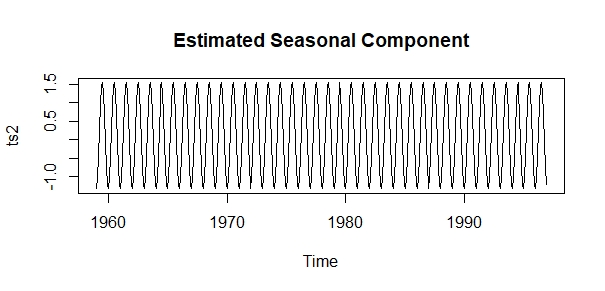
\includegraphics[width=10cm,height=5cm]{p41b.jpeg}
  %\caption{}
\end{figure}
Features:\\
All the estimated coefficients are significant.\\
The trend component is estimated to be convex, so the increasing rate (the slope) increases. It is not stationary.\\
The mean of the seasonal component is 0.1055 and the variance is 1.04503. It is stationary.\\

\item
R codes:
\lstinputlisting{p42a.R}
R outputs:
\begin{figure}[H]
  \centering
  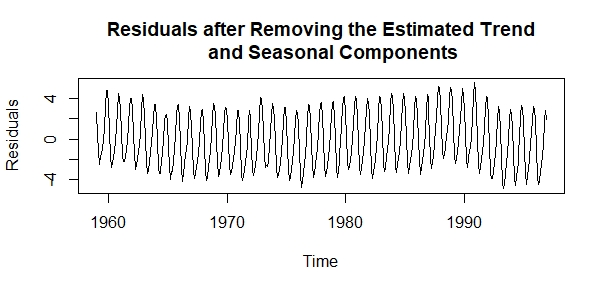
\includegraphics[width=10cm,height=5cm]{p42a.jpeg}
  %\caption{}
\end{figure}
Observation:\\
The trend has almost gone, but we can still see the dependence in the seasonal structure.

\item
R codes:
\lstinputlisting{p43a.R}
R outputs:
\begin{figure}[H]
  \centering
  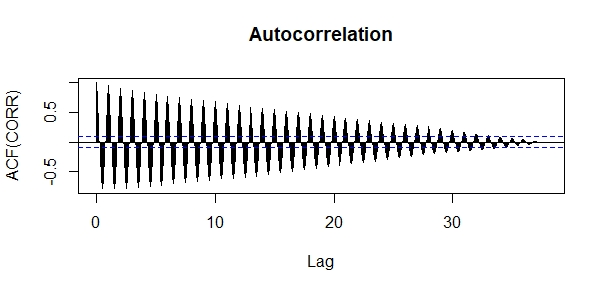
\includegraphics[width=10cm,height=5cm]{p43a.jpeg}
  %\caption{}
\end{figure}
\begin{figure}[H]
  \centering
  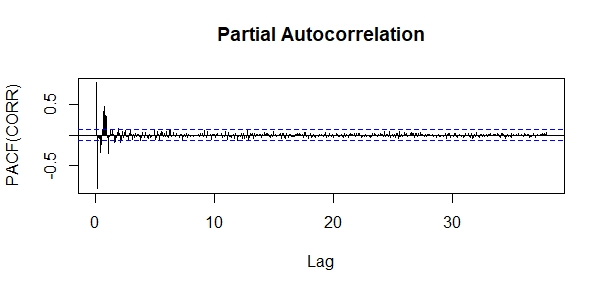
\includegraphics[width=10cm,height=5cm]{p43b.jpeg}
  %\caption{}
\end{figure}
Features:\\
The autocorrelation decreases as the lag increases; the partial autocorrelation is large at 1 and 2 lags and is around 0 after 2 lags.\\
Choice and explanations:\\
An AR(2) is probably appropriate, since the autocorrelation looks ``tails-off'' and the partial autocorrelation looks ``cuts-off'' after 2 lags.

\item
R codes:
\lstinputlisting{p44a.R}
R outputs:
\lstinputlisting{p44a.txt}
The equation form:
\begin{align*}
X_t&=1.6114X_{t-1}-0.892X_{t-2}+W_t
\end{align*}
The variance of the white noise process is 0.378.

\item
R codes:
\lstinputlisting{p45a.R}
R outputs:
\begin{figure}[H]
  \centering
  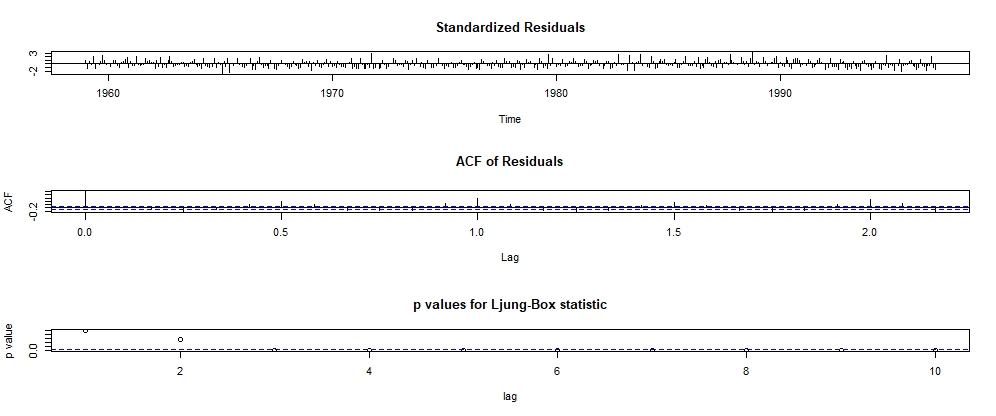
\includegraphics[width=12cm,height=7cm]{p45a.jpeg}
  %\caption{}
\end{figure}
Explanations:\\
The tsdiag function plots the standardized innovations $\frac{X_t-\hat{X}_t}{\sqrt{\hat{P}^{t-1}_t}}$, where $\hat{P}^{t-1}_t$ is the estimated one-step ahead prediction error. The standardized residuals for a good model should behave as a white noise sequence with mean zero and variance one.\footnote{ Scarrott, C. (2019). \textit{Lecture notes in time series methods}. Unpublished manuscript.}\\
In this case, through the Ljung-Box test in the plot, the p-values are small (close to 0), which lead to the recjection of $H_0$: $W_t$ is white noise, suggesting they are not white noise. Therefore, this model is not ideal.

\end{enumerate}

\end{document}
